\documentclass[11pt, twocolumn]{article}
\usepackage[german]{babel}
\usepackage[utf8]{inputenc}
\usepackage{graphicx}
\usepackage{hyperref}



\title{Lösungsansatz für den InformatiCup 2020}
\author{Jonas Peeters\\Nordakademie}

\begin{document}
\maketitle
\tableofcontents

\section{Beschreibung der Aufgabe}
In dieser Sektion soll die diesjährige Aufgabe des InformatiCup kurz beschrieben werden.

Dem Spieler wird eine feste Liste an Städten übergeben. Zu Beginn des Spieles brechen in einigen dieser Städte Krankheiten aus, die sich über mehrere Runden auch in andere Städte ausbreiten können. Zusätzlich finden noch verschiedene zufällige Ereignisse statt. Der Spieler kann dann unterschiedliche Züge durchführen, wie zum Beispiel Impfstoffe oder Medikamente entwicklen und den Städten verteilen.

Das Ziel des Spielers ist es, in möglichst wenigen Runden alle Krankheiten vollständig zu bekämpfen. Der Spieler verliert, wenn mehr als die Hälfte der Bevölkerung an den Krankheiten gestorben ist.

Die genauen Aktionen, die ein Spielen ausführen kann, sowie alle Spielregeln sind im bereitgestellten Dokument von der Gesellschaft für Informatik nachzulesen. 


\section{Neurale Netzwerke}
Zur Lösung der Aufgabe sollen künstliche Intelligenzen in Form von neuralen Netzwerken verwendet werden. Die genaue Umsetzung dieser ist in der Sektion Lösungsansätze beschrieben. In dieser Sektion wird die Funktionsweise von neuralen Netzwerken beschrieben. Dabei wird zwar die Funktionsweise von neuralen Netzwerken im Allgemeinen, jedoch mit starkem Focus auf die, in den Lösungsansätzen verwendeten, Konzepte, behandelt.

Neurale Netzwerke sollen im Grunde die Funktionsweise des menschlichen Gehirns modellieren, nehmen dabei aber einige Einschränkungen und Abwandlungen vor. Den Grundbaustein bilden dabei Neuronen.

\subsection{Neuronen}
\subsubsection{Im menschlichen Gehirn}
Neuronen haben einerseits die Möglichkeit Informationen von anderen Neuronen zu empfangen und andererseits die Möglichkeit Informationen an anderer Neuronen zu senden. Im menschlichen Gehirn findet dies über Dendrite statt, welche elektrische Impulse leiten. Wenn biologische Neuronen elektrische Impulse empfangen, so baut sich mit der Zeit eine elektrische Spannung zwischen der Innen- und Außenseite auf. Überschreitet diese Spannung dann irgendwann einen spezifischen Schwellwert, so wird ein elektrischer Impuls an alle Neuronen gesendet, die mit dem Ausgang dieses Neuronen verbunden sind.

\subsubsection{Schwellwerte}
Durch häufiges Verwenden eines Neuron verändern sich die Schwellwerte und mit der Zeit werden neue Verknüpfungen gebildet. Auf diese Art und Weise lernt das menschliche Gehirn.

Schwellwerte für die Inputs werden in einem neuralen Netzwerk Weights (Gewichtungen) genannt. Die Schwellwerte des Neuronen werden Bias (Neigungen/Verschiebungen) genannt.

\subsubsection{Aktivierungsfunktion}
In biologischen Neuronen ist die Stärke des ausgehenden Impulses zwar abhängig vom Input, im Normalfall jedoch nicht linear. Daher greift man auch bei der Simulation auf sogenannt Aktivierungsfunktionen zurück. Eine der häufigst genutzten ist die Sigmoid Funktion:
\begin{equation}
	\centering
	\frac{1}{1 + exp(-x)}
\end{equation}

\begin{figure}
	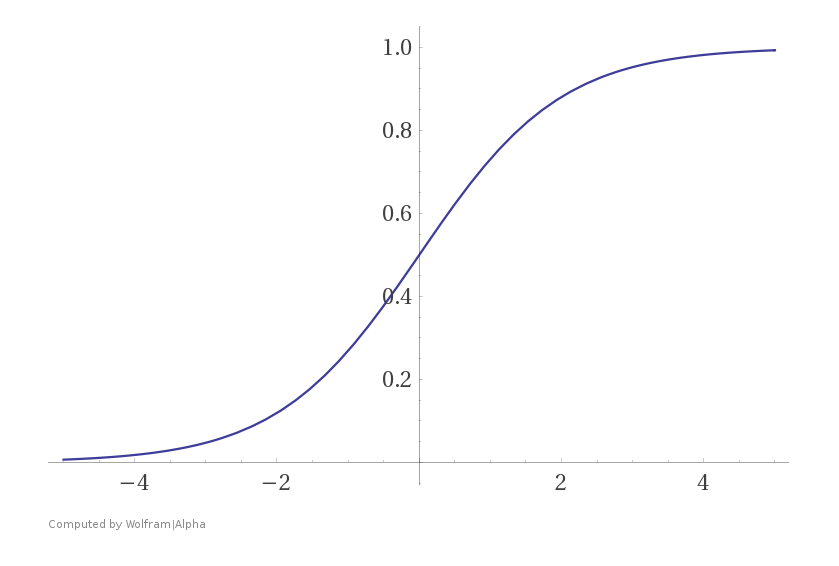
\includegraphics[width=\linewidth]{Sigmoid.png}
	\caption{Sigmoid Funktion in [-5;5] von WolframAlpha}
	\label{fig:sigmoid}
\end{figure}

Neben der Sigmoid Funktion werden aber auch gänzlich andere Funktionen verwendet. Diese reichen von einem tatsächlich linearen Verhalten bis zu einfachen Sinus oder Cosinus Funktionen.

Die Berechnungsformel für den Output eines Neuron mit $N$ Inputs $I_n$ welche die Gewichtungen $W_n$ haben mit dem Bias B lautet also:

\begin{equation}
	\centering
	sigmoid(B + \sum_{n=0}^{N}(I_n \cdot W_n))
\end{equation}
 
\subsubsection{Asynchron – Synchron}
Neuronen im menschlichen Gehirn arbeiten im Gegensatz zu den Neuronen in einem neuralen Netzwerk (NN) asynchron. Wie oben beschrieben baut sich über die Zeit die elektrischen Spannung auf.\footnote{Dies wird zum Teil aus in neuralen Netzwerken genutzt, hier verzichten wir allerdings darauf, da das Programm zustandslos arbeiten muss und dies dadurch gestört werden würde.}

Um die Berechnung im Computer möglich zu machen, bilden wir in einem neuralen Netzwerk Layers in welchen wir die Neuronen gruppieren.


\subsection{Layers}
Alle Neuronen einer Layer haben immer die Ausgänge der vorherigen Layer als Eingänge und die eigenen Ausgänge sind mit den Eingängen der nachfolgenden Layer verbunden. Dadurch können dann relativ einfach die Werte der Schichten nacheinander berechnet werden.

Alle Layers innerhalb eines Netzwerkes bezeichnet man normalerweise als Hidden Layers, da die genaue Art und Weise, wie diese Layers zur Lösung beitragen, nur sehr schwer nachvollziehbar ist.


\subsection{Training}
Da für die gestellte Aufgabe keine optimale Lösung bekannt ist, wird hier eine Trainingsmethode angewendet, welche als Reinforcement-Learning bezeichnet wird. Dazu werden in jeder Generation mehrere Netzwerke verwendet, die alle die selben Spiele (random Seed vom Spiel) spielen. Dies wird über mehrere Spiele getan, um verschiedene Szenarien zu testen.

Die Netzwerke werden dann bewertet. In diesem Fall wird dazu die benötigte Anzahl an Spielrunden verwendet, um zu gewinnen bzw. um zu verlieren. Bei verlorenen Spielen bekommen dabei die Netzwerke die höchste Bewertung, die am längsten durchgehalten haben. Bei gewonnen Spielen die, die die wenigsten Runden gebraucht haben.

Die besten Netzwerke kommen dann mehrfach in die nächste Generation, wobei die Weights und Biases zufällig angepasst werden. Dies wird solange fortgeführt, bis sich das Ergebnis nicht mehr verbessert.

\subsection{One Hot Representation}
Mithilfe der so bezeichneten One Hot Representation ist es möglich mithilfe von einem Neuralen Netzwerk eine Aktion, Klasse, etc. von mehreren zu selektieren. Gemeint ist zum Beispiel in der Klassifizierung von Fotos. Hier wird für jede mögliche Klasse ein Output Neuron festgelegt. Ein Foto ist dann in einer bestimmten Klasse, wenn das Output Neuron dieser Klasse den höchsten Wert zurück liefert. In der ersten Zeile von Abbildung \ref{tab:one-hot} würde zum Beispiel Klasse 3 ausgewählt werden.

Wenn auch mehrere Klassen ausgewählt werden können, so wird die mithilfe von Schwellwerten realisiert. In Zeile 2 könnten so Beispielsweise die Klassen 1 und 3 ausgewählt werden.

\begin{figure}[h]
\centering
\begin{tabular}{|r|c|c|c|c|}
	\hline
  	& Klasse 1 & Klasse 2 & Klasse 3 & Klasse 4 \\\hline
  	1 & 0.03 & 0.21 & 0.94 & 0.13 \\\hline
  	2 & 0.93 & 0.21 & 0.94 & 0.13 \\\hline
\end{tabular}
\caption{Beispielhafte Outputs eines Netzwerkes}
\label{tab:one-hot}
\end{figure}

Diese Form der Output Analyse wird in den Lösungsansätzen genutzt um zum Beispiel Aktionen und Städte für diese Aktionen auszuwählen.


\section{Lösungsansätze}
Ingesamt wurden zwei Lösungsansätze verfolgt. Zum einen wurde versucht ein großes Neurales Netzwerk zu trainieren, welches alle Informationen des Spiel erhält und davon ausgehend Aktionen ausführt. Zum anderen wurde ein Ansatz verfolgt, in dem das Problem auf kleinere einfachere Probleme heruntergebrochen wurde, welche dann von verschiedenen deutlich kleineren Neuralen Netzwerken gelöst werden.

\subsection{Ein großes neurales Netzwerk}
Um diesen Ansatz anzugehen wurde zunächst ein Konzept entwickelt, um den gesamten Spielstand in einem Array von Floats darzustellen, da ein solches letztendlich der Input für das Netzwerk sein muss. Bei dieser Erstellung wird jedoch bereits das erste große Problem schnell sichtbar. Da ein neurales Netzwerk zum Beispiel keine Events unterscheiden kann, müssen diese immer an den genau gleichen Stellen im Array abgelegt werden. Daher muss aber auch der Platz reserviert sein, wenn ein gegebenes Event gar nicht stattfindet. Dadurch wird der Input für das Netzwerk sehr schnell sehr groß.

Wenn der also Platz für jedes Event in jeder der 260 Städte berücksichtigt wird (und einige Events können mehrfach vorkommen), so sind wir in der Berechnung auf ca. 30.000 Inputs gekommen. Selbst wenn man diese direkt als Inputs auf 3.000 Neuronen in der ersten Layer mappt, so braucht man hierfür ca. 90.000.000 Weights. Bei 32 bit Floats werden also nur für die erste Layer 343 MB für die Gewichtungen benötigt. Wenn dann auch noch mehrere unterschiedliche Mutationen gleichzeitig trainiert werden sollen, sind die verfügbaren Ressourcen schnell erschöpft.

Dennoch wurde dieser Ansatz noch nicht verworfen. Da die ursprüngliche Implementierung in Python jedoch trotz der Nutzung von Numpy für schnellere Array Operationen zu langsam war, wurde die gesamte Codebase noch einmal in Swift implementiert. Hierbei wurden dann auch direkt die Array Operationen mit der Nutzung von Metal Compute Shadern auf die GPU verschoben.\footnote{Dies Funktioniert nur unter MacOS, ist allerdings auch nur für das eigentliche Training relevant, da für das tatsächliche Spielen die Zeit nicht so wichtig ist.}  Durch viele Optimierungen wurde die Geschwindigkeit deutlich erhöht. 

Letztendlich wurde jedoch auch über viele Spiele und Generationen kein Lernfortschritt erkennbar. Dies liegt wohl primär am zweiten großen Problem. Dieses Problem ist am Besten durch ein Beispiel erkennbar:

In Generation N ist in einem der Spiele in Stadt X ein Virus ausgebrochen und zufälliger Weise wurde am Ende der Generation das Netzwerk zu verändert, dass es besser auf diesen Virus hätte reagieren können. Wenn aber in Generation N+1 nicht zufälliger Weise in Stadt X der Virus ausbricht sondern in stattdessen in Stadt Y, so hat dieser Lernfortschritt dem Netzwerk nichts gebracht und wird vermutlich durch zukünftige Mutationen wieder zerstört.

Das grundsätzliche Problem ist also, dass das Netzwerk für jede einzelne der 260 Städte einzeln die Bekämpfung der Viren lernen müsste. Dies gilt zudem auch noch für alle anderen Events und wenn in einer Stadt ein zweiter Virus ausbricht, so muss dies auch extra gelernt werden. Aus diesem Grund ist tatsächlicher Lernfortschritt bei dieser Methode äußerst unwahrscheinlich.



\subsection{Mehrere kleine neurale Netzwerke}
Um die Probleme des großes Netzwerkes zu lösen wurde für diesen Ansatz das Problem in die folgenden kleineren Unterprobleme aufgeteilt:

\begin{enumerate}
	\item \textbf{Pathogen Prioritizer (PP)} \\
		Der PP erhält jeweils relevante Informationen über einen einzelnen Krankheitserreger und berechnet einen Prioritätswert. Für den Erreger mit der höchsten Priorität wird dann mit dem PAS eine Aktion ausgewählt.
	\item \textbf{Pathogen Action Selector (PAS)}\\
		Der PAS wählt über eine One Hot Representation zwischen Impfstoff und Medizin. Die manuelle Programmlogik überprüft dann ob bereits ein Impfstoff (bzw. Medizin) zur Verfügung steht. Ist dies nicht der Fall, so wird das entsprechende Mittel produziert. Wenn es bereits ein Mittel gibt, so wählt der PACS eine Stadt aus.
	\item \textbf{Pathogen Action City Selector (PACS)} \\
		Die Auswahl einer Stadt erfolgt über den PACS. Dieser erhält immer nur die Informationen einer Stadt, der gewünschten Aktion und des Erregers. Die Rückgabe ist dann erneut ein Prioritätswert. In der Stadt mit der höchsten Priorität wird dann der Impfstoff bzw. die Medizin verteilt.
	\item \textbf{City Selector (CS) und City Action Selector (CAS)}\\
		Wenn alle Erreger nur einen sehr niedrigen Prioritätswert haben, so wählt der CS eine Stadt aus, in der eine der übrigen Aktionen ausgeführt werden könnte. Der CAS bestimmt dann erneut über eine One Hot Representation, welche Aktion ausgeführt wird.
\end{enumerate}

Für eine genauere Betrachtung der Funktionsweise können die Dateien Logic.swift und GameState.swift angeschaut werden. In diesen ist die Struktur der Anwendung der Netzwerke, die Form der Eingabe und die Interpretation der Ausgabe einfacher zu erkennen, als ein Versuch, diese hier niederzuschreiben es vermöge.

Diese kleineren Netzwerke lösen die Probleme, die das große Netzwerk hatte. Zum einen sind sie deutlich kleiner. So haben alle Weights und Biases des PP zusammen gerade mal eine Größe von unter 1,4 KB. Das macht nicht nur die Berechnungen schneller, wodurch mehr Generationen berechnet werden können, sondern es gibt auch weniger Variablen, an die durch zufällige Mutationen einen guten Wert erreichen müssen.

Das zweite Problem ist ebenfalls gelöst. Da alle Städte immer vom gleichen Netzwerk bewertet werden, müssen die korrekten Variable-Belegungen nicht für jede Stadt neu gelernt werden.

\section{Geschwindigkeitsoptmierungen}
Damit der Lernprozess möglichst gut funktioniert und möglichst viele Spiele pro Generation und möglichst viele Generation durchgerechnet werden können, wurde an vielen Stellen versucht den Code zu optimieren. Einige davon werden hier beschrieben:

\begin{enumerate}
	\item \textbf{Verwendung von Numpy} \\
		Die Python Library Numpy bieten einen gewaltigen Geschwindigkeitsvorteil bei Operationen über große Array, wie zum Beispiel jedes Element einer Spalte in einem 2d Array mit der Korrespondierenden Spalte in einem 1d Array zu multiplizieren. Dieser Geschwindigkeitsvorteil liegt einerseits an der Struktur der Arrays und andererseits an der direkten C-Implementierung vieler Funktionen.
	\item \textbf{Wechsel von Python zu Swift} \\
		Da Python als interpretierte Sprache auf einer deutlich höheren Ebene über der CPU läuft als Swift, ist nur logisch, dass es nicht so schnell läuft wie Swift. Die ursprüngliche Geschwindigkeitssteigerung war jedoch nicht so hoch wie erwartet, aufgrund der sehr guten Optimieren von Numpy Array-Operationen.
	\item \textbf{Metal Compute Shader}\\
		Durch den Wechsel zu Swift hat sich die Option aufgetan Metal Compute Shader für die Array Multiplikation und die Generation vieler Zufallszahlen zu verwenden. Dadurch wurde die Geschwindigkeit etwa verdoppelt. Zahlreiche spätere Optimierungen, zum Beispiel beim Kopieren der Gewichtungen auf die GPU, haben die Geschwindigkeit nochmals deutlich erhöht.
	\item \textbf{Wechsel des Webservers}\\
		Bis zu diesem Zeitpunkt wurde der Perfect Webserver verwendet. Nach den Zahlreichen Optimierungen wurde dieser aber mittlerweile zum langsamsten Teil und hat ca. 50\% der gesamten Berechnungszeit pro Aktion gebraucht. Nach Tests mit Zahlreichen anderen Webservern, viel die Wahl letztendlich auf Kitura von IBM.
\end{enumerate}

Durch die oben benannten (und noch zahlreiche weitere kleinere) Optimierungen können bis zu 200 Aktionen pro Sekunde berechnet werden, was ca. 1 - 1,5 Spielen pro Sekunde entspricht. Um die volle Geschwindigkeit zu nutzen, müssen jedoch mehrere Spiele parallel gespielt werden, sodass während des Trainings immer 30 bis 50 Clients parallel liefen.

Es könnten sicher noch einige weitere Optimierungen vorgenommen werden. Tests haben aber gezeigt, dass ab ca. 250 bis 300 Aktionen pro Sekunde die CPU-Last der Clients überhand nimmt. An diesem Punkt müsste also der Client von der GI schneller gemacht werden, damit die Optimierungen noch zielführend sind.

\section{Weitere Aspekte}
\subsection{Architektur}
In der Main-Datei wird der Webserver erstellt und gestartet, nachdem alle Argumente entsprechen verarbeitet wurden. Kommt eine neue Anfrage an, so wird aus dieser zunächst einmal ein GameState erstellt, der im Grunde nur die Anfrage in From von nativen Swift Klassen ist. Als nächstes wird dieser GameState der Logik übergeben. Diese erstellt dann Eingaben für die Netzwerke, wertet diese aus, und erstellt daraufhin die nächste Aktion, welche dann zurück an den Client gesendet wird.

\subsection{Software Testing}
Mithilfe des XCTest Frameworks von Xcode werden unter anderem die relevantesten Funktionen der neuralen Netzwerke auf die Korrektheit überprüft. Da dies der Standardweg für Unit-Tests in Swift ist, wird auf eine Begründung verzichtet. Die Arbeitsweise der Netzwerke selber kann aber logischerweise nicht im klassischen Sinne getestet werden.

\subsection{Coding Conventions}
Primär wurde versucht sich an die \href{https://swift.org/documentation/api-design-guidelines}{Swift API Design Guidelines} zu halten. Es wurde allerdings an ein paar Stellen davon abgewichen, wenn es aus bestimmen Gründen sinnvoll war.

\subsection{Wartbarkeit}
Da der Projektumfang nicht sehr groß ist wurde nicht besonders auf hohe Wartbarkeit geachtet. Dennoch sind die einzelnen Module so weit Modularisiert wie sinnvoll war. Dazu kommt noch, dass natürlich bei jeder Änderung der Logik die Netzwerke sowieso neu trainiert werden müssen und daher die Wartbarkeit von vornherein eingeschränkt ist.

\section{Auswertung}
Um die Mutationen zu bewerten, wurde ein Punktesystem erstellt. Wurde das Spiel verloren, so erhält die Mutation so viele Punkte, wie das Spiel Runden gehabt hat. Wird das Spiel gewonnen, so ist die Punktzahl 300 abzüglich der Anzahl der Runden.

Werden ausschließlich EndRoundActions gesendet, so werden etwa 30\% der Spiele gewonnen. Mit den trainierten Netzwerken wurde dieser Wert auf ca. 50\% - 55\% erhöht. Die Punktanzahl wird im Schnitt um ca. 90 erhöht.


\section{Verbesserungsmöglichkeiten}
Es gibt verschiedene Ansätze den Server zu verbessern, welche allerdings aus Zeitgründen nicht versucht wurden. So könnte eine Änderungen der Trainingsparameter und längere Trainingszeiten die Güte der Netzwerke erhöhen.

Einen größeren Schub würde aber vermutlich eine veränderte der Logik für Ein- und Ausgabe der Netzwerke schaffen. Das aktuelle System ist relativ restriktiv, was die Freiheiten der KI betrifft, um die Trainingszeiten zu verkürzen. Mit einem offeneren System könnte dies aber besser funktionieren.


\end{document}






















